


\documentclass[10pt]{article}

\usepackage{xcolor}
\usepackage{cite }
\usepackage{graphicx, epsfig}
\usepackage[margin=1in]{geometry}
\usepackage[hyphens]{url}
\usepackage{enumitem}
\usepackage{amsmath}
\usepackage{algorithm}
\usepackage{algorithmic}

\pagenumbering{gobble} %Do not print page numbers

\newcommand\ceg[1]{\textcolor{red}{#1}} % Red marker to declare errors.

\begin{document}

\title{University of Florida Knowledge Base Acceleration Notebook}

%\numberofauthors{3}




\author{Morteza Shahriari Nia, Christan Grant, Yang Peng, Daisy Zhe Wang\footnote{University of Florida, Gainesville, Florida, USA}\\
       {\{msnia, cgrant, ypeng, daisyw\}@cise.ufl.edu}
\and
  Milenko Petrovic\footnote{Institute for Human and Machine Cognition, Ocala, Florida, USA}\\
       {mpetrovic@ihmc.us}
}

 \date{}

\maketitle



\begin{abstract}

% TODO this can be updated at the end

In this paper we will present the system design and algorithm adopted by the 
GatorDSR team, University of Florida to efficiently process TREC KBA 2013 --- 
SSF track. Here we will describe the system as well as the details 
the algorithms used to extract slot values for the given slot name. Scalability, efficiency, precision and recall are the major goals of this work, 
given the overly limited time limitation and available computational resources.

\end{abstract}



\section{Introduction}


In this paper we develop an efficient query-driven slot value extraction for given Wikipedia.org (WP) entities from a timely stream of documents on internet as they are being created. Slot value extraction is formally defined as follows: match each sentence to the generic sentence structure of [\textit{Subject} - \textit{Verb} - \textit{Adverbial/Complement}]\cite{sentencePatterns08}, where  \textit{Subject} represents the entity and \textit{Verb} is the relation type we are interested in (e.g. Table~\ref{table:slotNameOntology}). If a sentence matches these two components of the sentence pattern, \textit{Adverbial/Complement} would be returned as the other side of the relation (which we refer to as slot value). Slot value extraction is a challenging task in current state of the art Knowldge Bases (KB). Popular graphical KB such as Freebase or DBPedia keep data in structured format where entities are connected via relationships (\textit{Verb}) and the associated attributes (\textit{Adverbial/Compelement}). Our system can be used to automatically populate such KBs or even fill-in the information boxes at entity WP page itself.

Entities from three categories of \textit{person}, \textit{organization} and \textit{facility} are considered. The challenges that we address are: first finding documents that contain useful information about the entity (avoid spams, documents that do not have direct information about the entity even though they mention them, etc), the scale where \textit{stream processing} nature of the system makes it suitable to avoid batch processing natures of Hadoop and operate in the realm of streams such as twitter storm\footnote{http://storm-project.net/} which similarly processes unblounded streams of twitter data or Spark Streaming \footnote{http://spark.incubator.apache.org/}. Further, this is called streaming because data is being generated as time goes
on and for each extraction we should only consider current or past data. As other Natural Language Processing tasks, precision and recall of the extent we can extract slot values are very important metrics that we will discuss later on. Having to balance between infamous and obscure enitities, dealing with slots that can be very broad (e.g. things that an entity is affiliated with) or very specific (such as cause of death of a \textit{person} entity).

To take on an example assume we are analyzing a sentence from the internet such as "\underline{Boris Berezovsky} made his fortune in Russia in the 1990s when the country went through privatisation of state property and 'robber capitalism', and passed away March 2013.". First we have to pay attemtion that there are two \textit{Boris Berezovsky} entities in WP, one a businessman and the other a pianist. Any slot value extraction shall take this into account and try to come up with a viable distinguishing policy (Entity Resolution). Then, we match the sentence to find a slot value such as \textit{DateOfDeath} valued at March 2013. Other examples that this system can answer could be 'Who a person has met during a certain period of time?', 'Who are the employees of this organization?', 'Who has met who in this facility at a certain time?'.

 An important challenge in maintaining WP, the most popular web-based, collaborative, multilingual KB on the internet, is making sure its contents are up-to-date. Presently, there is considerable time lag between the publication date of cited news and the date of an edit to WP creating the citation. The median time lag for a sample of about 60K web pages cited by WP articles in the \textit{living\_people} category is over a year and the distribution has a long and heavy tail \cite{JFrank12}. Also, the majority of WP entities have updates on their associated article much less frequently than their mention frequency. Such stale entries are the norm in any large KB because the number of humans maintaining the KB is far fewer than the number of entities. %Further, the number of mentions is much larger than the number of entities~\cite{JFrank12}. 
Reducing latency keeps KBs and WP relevant and helpful to its users. Given an entity page, possible citations may come from a variety of sources. The actual citable information is a small percentage of the total documents that appear on the web. We develop a system to read streaming data and filter out articles that are candidates for citations. 

Our system contains three main components. First, we pre-process the data and build models representing the KB entries. Next, we use the models to filter a stream of documents so they only contain candidate citations. Lastly, we processes sentences from candidate extractions and return slot values. 
% EITHER SAY WHAT IT MEANS OR GIVE EXAMPLES OR COMMENT IT
%We build a modular system that allows us to explore the nuances of the training data and queries. 
Overall, we contribute the following:
\begin{itemize}[noitemsep,nolistsep]
\item Introduce a method to build models of name variations
\item Built a system to filter a large amount of diverse documents
\item Extract, infer and filter entity-slot-value triples of information to be added to KB 
\end{itemize}

\begin{table}
\caption{Ontology of Slots }
\centering
\label{table:slotNameOntology}

\begin{tabular}{|c|c|c|}
\hline 
\textbf{PER} & \textbf{FAC} & \textbf{ORG} \\ 
\hline 
\begin{tabular}{@{}l@{}}Affiliate \\ AssociateOf \\ Contact\_Meet\_PlaceTime \\ AwardsWon \\ 
DateOfDeath \\ 
CauseOfDeath\\
Titles\\
FounderOf\\
EmployeeOf\end{tabular}
  &
   \begin{tabular}[b]{l}Affiliate \\ Contact\_Meet\_Entity \end{tabular} 
   & 
   \begin{tabular}{@{}l@{}}Affiliate \\ TopMembers \\ FoundedBy\end{tabular} \\ 
\hline 
\end{tabular} 
\end{table}
% Evaluation Criteria


% Quick Discussion of our approach




\begin{figure}
\centering
%
\includegraphics[width=4.5in]{./images/system.eps}
\includegraphics[width=6in]{./images/SystemBW.eps}
\vspace*{-.1in} \caption{Pipeline Design }\label{fig:system}
\vspace*{-.2in}
\end{figure}

\section{System Overview}

In this section, we sketch out the main components of the system. Our system is built with a pipeline architecture in mind which gives it the advantage to run each section separately and allow stream processing without resources being wasted by one operation while others are awaiting (Figure \ref{fig:system}). This consists of a section to perform pre-processing to prepare the required data, Cumulative Citation Recommendation to annotate cite-worthy documents, Streaming Slot Filling which generates the actual slot values and Post processing to increase precision/recall. 

%\ceg{Discuss current system first. If you want to keep the decisions points that led to the current architecture, make it a subsection.}

\subsection{Preprocessing}

To begin, we need to have real-world aliases of entities of interest. TREC KBA prohibits Wikipedia entities to have any manual aliases being added and only allows automatic ways. We use Wikipedia API backlink references (redirects to a wiki entity) as aliases of the entity. We also use some techniques to extract  aliases from within the text of a wiki entity, which will be described later on. This whole process is referred to as \textit{Alias Extraction (Wiki API, Wiki text)}. On the other hand, regarding Twitter entities this limit is lifted and participants are allowed to manually add aliases for them. Part of the reason is that Twitter environment is composed of so much informal and dialectic language which makes it extremely difficult to extract alias out of tweets or entities descriptions in their profiles. This process of extracting aliases for Twitter entities is referred to as \textit{Manual Alias Extraction (Twitter)}.

Once aliases are available we pass them through some rules of generating proper name orders which will produce various forms of writing a name. As a basic example Bill Gates can be written as Gates, Bill. This will allow the system to capture various notation forms of aliases. We refer to this part as \textit{Name Order Generator}.

\subsection{CCR}

The main goal of Cumulative Citation Recommendation is to have an aggregate list of documents that are worthy of being cited in a Wikipedia page. Regarding CCR we perform exact string matching 
and treat all the documents that mention an entity equally likely to be citable.
For future iterations of the paper we have ideas on how to score documents 
based on their likelihood of citation worthiness, but for this iterations we 
treat all mentioning documents equally likely. One of the reasons for this is 
that in former TREC KBA reports \cite{JFrank12} there were observations of how 
non-mentioning documents have highly low chance of being citable in Wikipedia.
So we take on that and ignore non-citing documents. Regarding mentioning but 
garbage, neutral or central documents we produce more slot values which can be 
later on filtered out in the high accuracy filter section.

Our pipeline of processing the corpus consists of a two layer indexing system referred to as \textit{Chunk Files Index Generator} and \textit{StreamItems Index Generator}.  Chunk Files Index Generator will generate indexes of the chunk files that contain a mention of any of the desired entities. StreamItems Index Generator on the other hand will index StreamItems that contain a mention of a given entity respectively. This two level indexing will eliminate the need to process each and every ChunkFile/StreamItem for every entity. 



% Note: Describe the algorithms of each phase
% Talk in abstract terms not implementation.
% Use formal representations (Math, SQL etc)


%\ceg{This section should be structured as follows:
%1: Introduce CCR (Motivation, Expectations)
%2: Our high level approach
%3: Discussion of our design (Like already discussed)
%}


\subsection{SSF}
%\ceg{See the previous note.}
As described in the Introduction, the general purpose of slot filling is to extract proper values for relations of interest, some of which can be found in Table \ref{table:slotNameOntology}. This is called Stream Slot Filling due to the fact that it is assumed that data is being generated as time goes on and for each extraction we should only consider current or past data. In our schematic diagram we refer to this as \textit{Streaming Slot Value Extraction}. Stream slot filling is done by pattern matching documents with manually 
produced patterns for slots of interest. The way we do this is by observing a 
sentence that has a mention of the entity or one of its coreferences. An 
anchor word in the sentence related to the slot name is located and we match 
either left or right of the anchor word for potential slot values. 

\subsection{Post Processing Algorithm}

The SSF output of many extractions is noisy. The data contains duplicates and 
incorrect extractions. We can define rules to sanitize the output only using 
the information present in the SSF file. The file is processed in time order, 
in a tuple-at-a-time fashion to minimize the impact on accuracy. We define 
two classes of rules deduplication rules and inference rules. In our diagram we refer to this component as \textbf{High Accuracy Filter}.




\section{Implementation}
\label{section:implementation}

We extract aliases for entities from Wikipedia automatically both using API 
and using the actual page content, then apply pattern matching rules for slot 
value extraction. Our contribution is that we perform pattern matching that conforms to each slot 
value along with post-processings to eliminate noisy outputs. 

%\ceg{Instead of this paragraph we talk about what this %section will
%contain. We can discuss the input/output of the system %too.
%}

\subsection{Alias Generation}
\label{section:aliasgeneration}

We use Wikipedia API to get some aliases automatically. This is done by 
retrieving backlink references (redirects of a wiki entity). Unfortunately 
this is not good enough and to enhance recall we need more aliases. To have 
better use of a wiki page we parse HTML DOM of the page, then use regular 
expressions to extract the bold phrases of the first paragraph as alias of the 
actual entity. Based on our observation this is a very accurate heuristic and 
provides us with lots of famous aliases of the entities. To consider other 
typical cases we consider some generic first name last name order swapping 
conventions such as Bill Gates $\rightarrow$ Gates, Bill.  Meanwhile, William Henry
Gates is an alias for Bill Gates in WP as a backlink reference. These kinds of
aliases are also included in matching entities. 

\subsection{Cumulative Citation Recommendation}
\label{sec:ccrimpl}

Our pipeline of processing the corpus consists of a two layer indexing system 
referred to as \textit{Chunk Files Index Generator} and \textit{StreamItems Index Generator}.
Chunk Files Index Generator will generate indexes of the chunk files 
that contain a mention of any of the desired entities. StreamItems Index Generator 
on the other hand will index StreamItems that contain a mention of a given entity 
respectively. This two level indexing will eliminate the need to process each and 
every ChunkFile/StreamItem for every entity. The reason for splitting this task 
into two steps is that not all chunk files contain any mention of the entities and 
we want to get rid of them as soon as possible. Chunk Files Index Generator which 
is written in C++ discards non-mentioning chunk files and will stop further 
processing a chunk file as soon as it finds a mention there. Each chunk file can 
contain up to thousands of SIs which can be so time consuming if we were to 
process them in our Java base code. Processing StreamItems on the other hand is 
done in Java with ideas in mind for later on extensibility by adding other Java libraries.



\subsection{Streaming Slot Value Extraction}
\label{sec:ssve}
\begin{figure}
\centering
%
\includegraphics[width=4.5in]{./images/system.eps}
%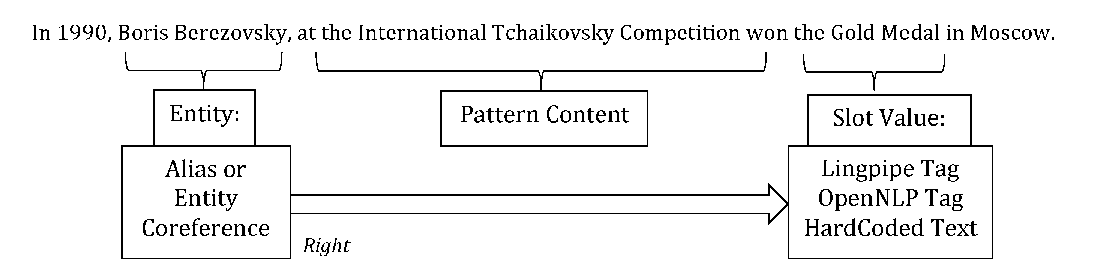
\includegraphics[width=6in]{./images/Pattern.eps}
%\includegraphics[width=6in]{./images/Pattern-eps-converted-to.pdf}
\includegraphics[width=6in]{./images/Pattern-crop.pdf}
% cropped pdf created using $ pdfcrop Pattern.pdf
\vspace*{-.1in} \caption{Pattern Matching with Slot Value on the Right Side of Entity. }\label{fig:pattern}
\vspace*{-.2in}
\end{figure}

In the data set, we are given 4 months of data (October 2011 - February 2012) as training data.
Instead of building a classifier we use pattern matching methods to find
corresponding slot values for entities. 
Pattern matching is simple to manipulate results and implement.
Additionally, a classifier approach is more difficult to evaluate and explain results.

The procedure to extract slots with the patterns is to 
first find Streamitems that contain the
entities by using alias names of the entities. Next, inside these Streamitems, 
fetch the sentences which contain entities by using alias names and the 
coreference information provided by Lingpipe tags. Use these sentences to 
match existing patterns, and when patterns matched, generate SSF results.

\begin{algorithm}
  \caption{Streaming Slot Value Extraction Pseudocode}
  \textbf{List of entities $\mathcal{E} = \{e_0, \ldots, e_{170}\}$}\\
  \textbf{List of Streamitems $\mathcal{S} = \{s_0, \ldots, s_{|\mathcal{S}|}\}$}\\
  \textbf{List of patterns $P = \{p_0, \ldots, p_{|P|}\}$}\\
  \begin{algorithmic}%[1]
    \FOR{$si \in \mathcal{S}$}
      \FOR{$sentence \in si$}
        %%\IF{check\_pattern(sentence, pattern)}
        \FOR{$pattern \in P$}
          \IF{Satisfies($sentence$, $pattern$)}
            \STATE Emit($sentence$, $pattern$) // Deal specifically with the three types
          \ENDIF
        \ENDFOR
      \ENDFOR
    \ENDFOR
  \end{algorithmic}
\end{algorithm}


\subsubsection{Types of patterns}
A pattern is defined as a record representing knowledge going to be added to a knowledge base.
A pattern $\mathcal{P}$ is represented as a five-tuple $\mathcal{P} = \langle p_1, p_2, p_3, p_4, p_5 \rangle$.


The first value, $p_1$ represents the type of entity. These entity types are in
the set $\{ \text{\tt FAC}, \text{\tt ORG}, \text{\tt PER} \}$ where \texttt{FAC}
represents a type of facility, \texttt{ORG} represents an organization and \texttt{PER}
represents a person.
The $p_2$ represents a slot name.
A list of slot names is present in Table~\ref{table:slotNameOntology}.
The third element $p_3$ is the pattern content. This is a string found in the sentence.
The extractor looks for this exact string or pattern in a sentence.
The pattern evaluator uses a direction (\texttt{left} or \texttt{right}) found in
$p_4$ to explore sentence.
The final element $p_5$ represent the slot value of a pattern. Thois
%When we match one pattern, we match all the 
%fields except the third field, which is extracted as the final result.
The type of slot value may be the entity 
type tagged by Lingpipe, a noun phrase (\texttt{NP}) tagged by OpenNLP or a hard-coded phrase. 
For these three kinds of patterns, we implement them in different 
ways accordingly. Next, we explain the patterns with more details, an
example can be found in Figure~\ref{fig:pattern}. 

\textbf{Type I.} This pattern type is driven by the slot value type, a pattern
tagged by Lingpipe. For example, pattern
$\langle$\texttt{PER, FounderOf, \textit{founder}, right, ORG}$\rangle$. \texttt{PER} means 
that the entity we are finding slot values for a PER entity; \texttt{FounderOf} 
means this is a pattern for FounderOf slot. \textit{founder} is the anchor word we are 
match in a sentence; \texttt{right} means that we are going to the 
right part of the sentence to match the pattern and find the slot value; ORG 
means the slot value should be a ORG entity.

\textbf{Type II.} This pattern type is unique because it only looks for a
slot value tagged as noun phrase (NP) by OpenNLP.\@ For example,
pattern $\langle$\texttt{PER, AwardsWon, \textit{awarded}, 
right, NP}$\rangle$. This pattern can be interpreted 
as that we are looking for a noun phrase after the \textit{awarded} since that noun 
phrase may represent an award. Titles and awards are usually 
not the Lingpipe entities, hence the use of the OpenNLP noun phrase chunker to fetch the 
noun phrases.

\textbf{Type III.} Some relations are best discovered by hard coding the slot values.
Examples of these include time phrases: $\langle$\texttt{PER, DateOfDeath, \textit{died}, right, 
\textit{last night}}$\rangle$. In this pattern, \textit{last night} means we are looking for 
exactly the phrase \textit{last night} to the right of \textit{died}. This pattern is 
inspired by the intuition that in news articles, people often mention that 
somebody died last night instead of mentioning the accurate date information 
and Lingpipe tends not to tag phrases like \textit{last night} as a DATE entity. 

We sampled documents from the training data period to generate an initial set of patterns. We then use these patterns to generate SSF results. By manully looking at these results, we prune some patterns with poor­performance and add more patterns that we identified from these results. We use several iterations to find the best patterns. We found that it is time consuming to identity quality pattern.


We found three major classes of accuracy errors:
incorrect entities selected, incorrect tags by Lingpipe and incorrect pattern extractions.
The first issue is ameliorated by generating better aliases (Section~\ref{section:aliasgeneration}). And we use
post-processing to reduce the second and third types of errors (Section~\ref{section:highAccuracyFilter}).
We didn't use more advanced NLP packages such as Stanford NLP because of the large size of the data set.
The post-processing step to improve the results is discussed in the next section.

\subsection{High Accuracy Filter}
\label{section:highAccuracyFilter}

The SSF output of streaming slot value extraction is noisy. The data contains duplicates and 
incorrect extractions. We can define rules to sanitize the output only using 
the information present in the SSF file. The file is processed in time order, 
in a tuple-at-a-time fashion to minimize the impact on accuracy. We define 
two classes of rules: \textit{deduplication} and \textit{inference} rules.

The output contains many duplicate entries. As we read the list of extracted 
slots we create rules to define ``duplicate''. Duplicates can be present in a 
window of rows; we use a window size of 2 meaning we only be adjacent rows. 
Two rows are duplicates if they have the same exact extraction, or if the 
rows have the same slot name and a similar slot value or if the extracted 
sentence for a particular slot types come from the same sentence.

 New slots can be deduced from existing slots by defining inference rules. 
 For example, two slots for the task are ``FounderOf'' and ``FoundedBy''. A safe 
 assumption is these slot names are biconditional logical connectives with the 
 entities and slot values. Therefore, we can express a rule ``X FounderOf Y'' 
 equals ``Y FoundedBy X'' where X and Y are single unique entities. Additionally,
 we found that the slot names ``Contact\_Meet\_PlaceTime'' could be inferred as
 ``Contact\_Meet\_Entity'' if the Entity was a FAC and the extracted sentence 
 contained an additional ORG/FAC tag.  
We also remove erronious slots that have extractions that are several pages in 
length or tool small. Errors of extracting long sentences can typically be 
attributed to poor sentence parsing of web documents. We have some valid
``small'' extractions. For example a comma may separate a name and a title
(e.g. ``John, Professor at MIT''). But such extraction rules can be particularly 
noisy, so we check to see if the extracted values have good entity values.


% Note: Talk about how each of the algorithms were created

% Note: Give enough information for our algorithms to be
% reimplemented and verified.




\section{Results}

% Note: Here is where we give as much stats as possible on our runs





\section{Discussions}

%In this section we address some of the challenges that we faced during the course of this project. We started 
%off by trying to use the off-the-shelf tools for this task. We started 
%by using Scala/Spark~\cite{ferc11} to benefit from the parallelization 
%performance there. Unfortunately Spark was not performant and the distributed reliability overhead 
%was much more than tolerable. We moved on to use Scala parallelization  framework itself, and unfortunately it did not satisfy our needs as well; there was 
%excessive memory overhead on map-reduce jobs. We migrated the core of the 
%system to Java Parallelism APIs and that was not good enough either, we still demanded 
%better. So we built our own parallel system which in actual performance had 
%the least of overhead, the least memory consumption and the most robust memory 
%model which avoided unpredictable CPU stalls on garbage collections in 
%processing the corpus.

Table~\ref{table:finalresultrecall} shows the distribution of extracted slot names.
The number of extraction between slot names vary greatly.
Some slots naturally have more results than other slots.
For example DateOfDeath and CauseOfDeath have some of the fewest entities because only a few entities are deceased.
Some patterns use common words as as part of their patterns causing more extractions.
For example, Affiliate looks for common words like  \textit{and} and  \textit{with} as part of the pattern content.
These words are more common than \textit{dead}, \textit{died} or \textit{founded} in other patterns. 

%As part of future work regarding enhancing precision, we can focus on fixing the wrong entities found, remove noisy tags by the Lingpipe or use more accurate NLP taggers such as Stanford NLP (Due to the fact that Stanford NLP is very slow we avoided using it, as due to speed its use was out of question) and finally use better patterns to enahnce results matched by the patterns.
%On the other hand to increase recall we need to find better aliases and go for more resources to discover other ways that an entity might be addressed (e.g.\ twitter id, website, etc), add powerful patterns that can capture more cases of slot values. We would also use entity resolution methods and other advanced methods to improve 
%the accuracy and recall of entity extraction part. 

%For slot extraction, to improve the performance, we need: 1) Using multi-class classifiers instead of pattern matching method to extract slot values in order to increase both recall and accuracy for slots ``Affiliate'', ``AssociateOf'', ``FounderOf'', ``EmployeeOf'', ``FoundedBy'', ``TopMembers'', ``Contact\_Meet\_Entity'' and so on. 2) For special slots, like ``Titles'', ``DateOfDeath'', ``CauseOfDeath'', ``AwardsWon'', using different kind of advanced methods, e.g.\ classifiers, matching methods. 3) Using other NLP tools or using classifiers to overcome the drawbacks of the LingPipe’s inaccurate tags. The first and second tasks are the most important tasks we need to do.

Some of the entities are popular and appear at a greater frequency in the data set.
For example, a `Brenda Weiler' Google search results in 860,000 documents.
\ceg{Add an example of someone who is either much larger of smaller.}
For our small portion of the web it might make sense.
The histogram of the entities shows that more than half of the entities have appeared in less than 10 documents.
\ceg{Can we add this figure}
A large portion have appeared only once.

%A theory is that we are falling behind because we are using the cleansed (from HTML tags)
%version of the corpus. We believe there has been a reason that TREC has 
%included the actual HTML document as well as the cleansed version. This 
%definitely will convey some information to us. If it was as easy as reading 
%some clean text they wouldn't bother including so much data for teams to be 
%useless. So we guess is that we are missing some information from not using 
%the actual document. And, we are looking for tokens with entity value set 
%which will depend us dramatically on the accuracy of lingpipe, which is a fast 
%algorithm but is not as good as other NLP tools can be e.g. Stanford NLP.

% Note: Here we discuss why the results are the way they are
% Give pros and cons, talk about how the implemented algorithms
% performed in the actual implementation.
% Answer the `why' question about all the trends in the results section.




In this paper we described an approach to perform fact extraction over one of the largest data sets to date. 
We generate aliases for Wikipedia entities using an API and extract some aliases from Wikipedia pages text itself.
We process documents that mention entities for slot value extraction.
Slot values are determined using pattern matching over coreferences of entities in sentences. Finally post processing will filter, cleanup and infers some new slot values to enhance recall and accuracy. 

We sampled documents from the training data period to generate an initial set of patterns and then use these patterns to generate results.
After manually examining the results, we prune patterns with poor performance and add patterns that may add to extraction coverage.
We use several iterations to find the best patterns.
%We found that it is very time consuming to identify quality patterns.

%We noticed that some tools that claim to be performant for using the hardware capabilities at hand sometimes don't really work as claimed and you should not always rely on one without a thorough A/B testing of performance which we ended up in generating our in-house system for processing the corpus and passing through the filter. Furthermore, on extracting slot values, pattern matching might not be the best options but definitely can produce some good results at hand. We have plans on generating classifiers for slot value extraction purposes. Entity resolution on the other hand was a topic we spent sometime on but could not get to stable grounds for it. Entity resolution will distinguish between entities of the same name but different contexts. Further improvements on this component of the system are required. 


We look to continue exploration of streaming extraction models over this large data set.
Our models are simple and provide a great baseline framework to develop and compare innovative techniques.





\section{Conclusions}

We experimented through different tools and approaches to best process the massive amounts of data on the platform that we had available to us. We generate aliases for wikipedia entities using Wiki API and extract some aliases from wikipedia pages text itself. On twitter entities we extract aliases manually as it is part of the rule of the KBA track. We process   documents that mention entities for slot value extraction. Slot values are determined using pattern matching over coreferences of entities in sentences. Finally post processing will filter, cleanup and infers some new slot values to enhance recall and accuracy. 

We noticed that some tools that claim to be performant for using the hardware capabilities at hand sometimes don't really work as claimed and you should not always rely on one without a thorough A/B testing of performance which we ended up in generating our in-house system for processing the corpus and generating the index. Furthermore, on extracting slot values, pattern matching might not be the best options but definitely can produce some good results at hand. We have plans on generating classifiers for slot value extraction purposes. Entity resolution on the other hand was a topic we spent sometime on but could not get to stable grounds for it. Entity resolution will distinguish between entities of the same name but different contexts. Further improvements on this component of the system are required. 


% Note: Give a summary of our efforts and the
% high level contribution to society.

% Talk about the things we wanted to do and
% didnt get to do.



\section*{Acknowledgements}
Christan Grant is funded by a National Science Foundation Graduate Research
Fellowship under Grant No. DGE-0802270. This work has also been supported in part by DARPA under
FA8750-12-2-0348-2 (DEFT/CUBISM).

%\bibliographystyle{acm}
%\bibliography{citation}

\bibliographystyle{unsrt}
\bibliography{citation}



\appendix

\section{KBA Task Background}
\label{sec:kbatask}
The National Institute of Standards (NIST) hosted the
Text REtrieval Conference (TREC) --- Knowledge Base Acceleration challenge in 2013. The task
contains two main sections designed for this track, Cumulative Citation Recommendation 
and Streaming Slot Filling. Due to the importance of knowledge bases, both of these 
tracks aim to accelerating populating them, hence the title Knowledge Base Acceleration (KBA).
Below we describe each of these tracks and their purposes.

\subsection{Cumulative Citation Recommendation (CCR)}

For this track, assessors were instructed to ``use the Wikipedia article to 
identify (disambiguate) the entity, and then imagine forgetting all info in the WP 
article and asking whether the text provides any information about the entity'' \cite{JFrank12}.
Documents are divided according if an entity is mentioned and a relevance level to the entity.

More specifically, a document may have a mention or be without a mention.
\begin{itemize}[noitemsep]
  \item \textbf{Mention:} Document explicitly mentions target entity, such as full 
    name, partial name, nickname, pseudonym, title, stage name.
  \item \textbf{Zero-mention:} Document does not directly mention target. Could 
    still be relevant, e.g.\ metonymic references like ``this administration'' 
    $\rightarrow$ ``Obama''. See also synecdoche. A document could also be relevant to 
    target entity through relation to entities mentioned in document -- apply this 
    test question: can I learn something from this document about target entity using 
    whatever other information I have about entity?
\end{itemize}

The relevance of a document to a query is split into the four classifications.
\begin{itemize}[noitemsep]
  \item \textbf{Garbage:} not relevant, e.g.\ spam.
  \item \textbf{Neutral:} Not relevant, i.e.\ no info could be deduced about entity, 
    e.g., entity name used in product name, or only pertains to community of target 
    such that no information could be learned about entity, although you can see how 
    an automatic algorithm might have thought it was relevant.
  \item \textbf{Relevant:} Relates indirectly, e.g., tangential with substantive 
    implications, or topics or events of likely
    impact on entity.
  \item \textbf{Central:} Relates directly to target such that you would cite it in 
    the WP article for this entity, e.g.\ entity is a
    central figure in topics/events.
\end{itemize}


\subsection{Streaming Slot Filling (SSF)}
The task is that given certain WP or Twitter entities 
(wiki/twitter URLs) and certain relations of interest (given in
Table~\ref{table:slotNameOntology}), extract as many triple relations as possible (
hence, slot filling). This can be used to automatically populate knowledgebases 
such as free-base or DBPedia or even fill-in the information boxes at Wikipedia. 
Below, you can view some examples of what it means to fill in a slot value; in 
each example there is a sentence of interest that we wish to extract slot values 
from, an entity that the slot value is related to, and a slot name which can be 
thought of as the topic of the slot value:

\noindent \textbf{Example 1:} ``Matthew DeLorenzo and Josiah Vega, both 14 years old and students 
at Elysian Charter School, were honored Friday morning by C-SPAN and received 
\$1,500 as well as an iPod Touch after winning a nationwide video contest.''

Entity:  http://en.wikipedia.org/wiki/Elysian\_Charter\_School

Slot name: Affiliate

Possible slot values: ``Matthew DeLorenzo'', ``Josiah Vega''

Incorrect slot values: ``C-SPAN'', ``iPod Touch''

\noindent \textbf{Example 2:} ``Veteran songwriters and performers Ben Mason, Jeff Severson and 
Jeff Smith will perform on Saturday, April 14 at 7:30 pm at Creative Cauldron 
at ArtSpace, 410 S. Maple Avenue.''

Entity: http://en.wikipedia.org/wiki/Jeff\_Severson

Slot name: Affiliate

Possible slot values: ``Ben Mason'', ``Jeff Severson'', ``Jeff Smith''

Incorrect slot values: ``Creative Caldron'', ``Art Space''

\noindent \textbf{Example 3:}  ``Lt. Gov. Drew Wrigley and Robert Wefald, a retired North Dakota 
district judge and former state attorney general, unveiled the crest Friday 
during a ceremony at the North Dakota Capitol.''

Entity: http://en.wikipedia.org/wiki/Hjemkomst\_Center

Slot name: Contact\_Meet\_PlaceTime

Slot value: ``Friday during a ceremony at the North Dakota Capitol''


\noindent In \textit{streaming} slot filling, we are only interested in new 
slot values that were not substantiated earlier in the stream corpus.
In Table~\ref{table:slotNameOntology} you can view some slot values 
and their types, the comprehensive description of which can be found at
\cite{tackbp} and \cite{aec}. The details of the metric for SSF will favor systems 
that most closely match the changes in the ground truth time line of slot values. 
This is done by searching for other documents that mentioned an entity and exactly 
matched the slot fill strings selected by the assessors.



%In the rest of the paper, we address the following material. In Section 2, we 
%sketch the main components of the system and their purposes. In Section 3, 
%describe the details of how we designed and implemented certain components 
%critical to the behavior of the system. Section 4 addresses the performance and 
%the results we achieved. Section 5, goes through a discussion of the challenges we 
%had to produce reliable results over the massive amount of information available, 
%and how we overcome these issues.
For similar approaches regarding last year's track you can refer to \cite{ji2011knowledge}.

%\ceg{Add a discussion of why machine driven kb population is important.}


\begin{table}[h]
\caption{Ontology of Slot Name Categories }
\centering
\label{table:slotNameOntology}

\begin{tabular}{|c|c|c|}
\hline 
\textbf{PER} & \textbf{FAC} & \textbf{ORG} \\ 
\hline 
\begin{tabular}{@{}l@{}}Affiliate \\ AssociateOf \\ Contact\_Meet\_PlaceTime \\ AwardsWon \\ 
DateOfDeath \\ 
CauseOfDeath\\
Titles\\
FounderOf\\
EmployeeOf\end{tabular}
  &
   \begin{tabular}[b]{l}Affiliate \\ Contact\_Meet\_Entity \end{tabular} 
   & 
   \begin{tabular}{@{}l@{}}Affiliate \\ TopMembers \\ FoundedBy\end{tabular} \\ 
\hline 
\end{tabular} 
\end{table}


%\ceg{How will each submission be evaluated?}

% Motivation


% KBA Task






\end{document}
